\documentclass[11pt,a4paper]{article}
\usepackage[top=3cm, bottom=3cm, left=2.5cm, right=2.2cm]{geometry} %geometry of page
\usepackage[hidelinks]{hyperref} %reference links
\usepackage{fancyhdr} %header and footer control
\usepackage{minted} %source code syntax highlighting
\usepackage{qrcode} %qrcode links
\usepackage{graphicx} %images
\usepackage{tikz} %diagrams
\usepackage{subcaption} %sub-figures
\usepackage{parskip}
\usetikzlibrary{calc}

\linespread{1.3}
\emergencystretch 3em

% Set Header and Footer
\fancyhead{}
\fancyhead[L]{\textbf{Lab 4: Hall effect sensor}}
\fancyhead[R]{max.champneys@sheffield.ac.uk}
\fancyfoot{}
\fancyfoot[L]{\thepage}
\fancyfoot[R]{MAC 233 Arduino Labs, School of MAC, University of Sheffield}

% Create Document
\begin{document}
\pagestyle{fancy}

\section*{Prerequisites}
This lab doesn't require any code from previous labs; however, it does expect you to have completed these, as common code repeated from previous labs will not be explained in detail again here. Out of your Arduino pack, you will need: 1 Arduino, 1 breadboard, 1 A3144 hall effect sensor, 1 magnet, 1 LED, 1 $10K\Omega$ resistor, 1 $220\Omega$ resistor, and 5 jumper cables.

\section*{Objectives}
The objective of today's lab is to learn how to use an interrupt to record a value of a sensor whose value is changed via an external event: \url{https://docs.arduino.cc/language-reference/en/functions/external-interrupts/attachInterrupt/}.

This worksheet will take you through the steps of how to connect a hall effect sensor to your Arduino, monitor when the value of the sensor has changed, and provide visual feedback to an end user of when the value has changed.

\section*{Hall effect sensors}
In short, a hall effect sensor allows you to detect the presence of a magnet, the value given by the sensor changes when a magnet is near to it. This type of sensor has many applications, but most importantly for us, it provides a way to detect movement.

\begin{figure}[ht]
    \begin{center}
        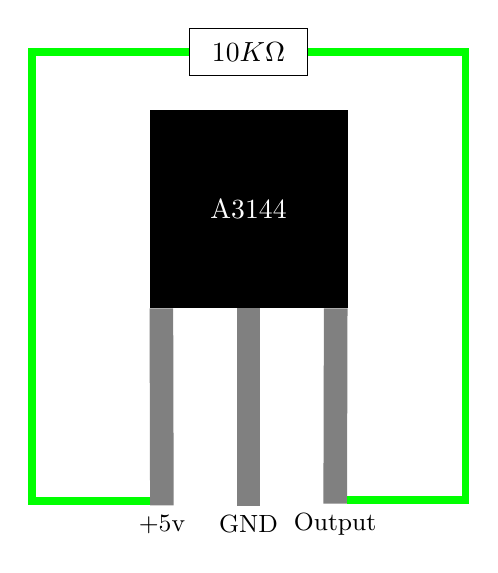
\begin{tikzpicture}[
            sensor/.style={fill=black, draw=black, text=white, minimum size=2.5cm},
            resistor/.style={fill=none, draw=black, text=black, minimum height=.6cm, minimum width=1.5cm},
            pin/.style={draw=gray, line width=3mm},
            wire/.style={line width=1mm},
            label/.style={draw=none, text=black},
        ]
            %% components
            \node[resistor] at (0, 2) (resistor) {$10K\Omega$};
            \node[sensor] at (0, 0) (hall-effect){A3144};
            \node[label] at (-1.1, -4) (positive) {\small +5v};
            \node[label] at (0, -4) (ground) {\small GND};
            \node[label] at (1.1, -4) (output) {\small Output};
            %% pin
            \draw[pin] ($(hall-effect.south west) + (0.15, 0)$) -- (positive);
            \draw[pin] (hall-effect.south) -- (ground);
            \draw[pin] ($(hall-effect.south east) - (0.15, 0)$) -- (output);
            %% connection
            \draw[wire, draw=green] let \p1 = ($(positive.north) + (-0.155, 0.05)$), \p2 = ($(\p1) - (1.5, 0)$), \p3 = (resistor.west) in (\p1) -- (\p2) -- (\x2, \y3) -- (\p3);
            \draw[wire, draw=green] let \p1 = ($(output.north) + (0.155, 0.05)$), \p2 = ($(\p1) + (1.5, 0)$), \p3 = (resistor.east) in (\p1) -- (\p2) -- (\x2, \y3) -- (\p3);

        \end{tikzpicture}
    \end{center}
    \caption{The connections for our hall effect sensor. The sensor has two bases on a trapezium; this diagram is drawn with the short base facing towards you.}
    \label{fig:hall-effect-sensor}
\end{figure}

The particular hall effect sensor you have in your kit has three legs: a \textit{power} leg, a \textit{ground} leg, and a \textit{digital output} leg. The sensor is shaped like a trapezium. With the short base of the trapezium facing towards you (as depicted in Figure \ref{fig:hall-effect-sensor}) and the legs facing south, the sensor is wired into the Arduino as follows: Arduino +5V\textrightarrow left leg, Arduino GND\textrightarrow middle leg, and Arduino Pin D2\textrightarrow right leg.

\section*{Interrupts}
The purpose of today's lab, is to gain experience of when and how to use an \textit{interrupt} in an Arduino. In previous labs, we have changed the value of an externally connected device using the command \verb|digitalWrite|. You can read the value of a sensor using the command \verb|digitalRead|; however, this method is not always appropriate when you consider when within the event timeline, the value of the sensor may change.

Let's consider how an Arduino works in context of an event timeline. The Arduino runs the code within the `setup' function, then runs the code in the `loop' function continuously until it is turned off. If we were to put as the first line of the `loop' function \verb|digitalRead(PIN)|, we could capture the value of pin at the beginning of the loop. The Arduino would then execute the rest of the code within the `loop' function, then start the `loop' again, at which point we would then capture the current value of the pin again. This is shown in Figure \ref{fig:polling}.

This design pattern works well in a system that is designed to monitor the gradual change of a value over a period of time (e.g. capturing the temperature outside every five minutes over a twenty-four-hour period) However, this design pattern fails in a scenario where the sensor value could have changed between the two instances of the \verb|digitalRead| logic. In this scenario you need a way of interrupting the Arduino to pause whatever it is doing, run the required code needed to record a value change, and then continue with its previous operations.

In Arduino, this functionality is called an \textit{interrupt}. Consider the event timelines in Figure \ref{fig:reading-a-pin}.

\begin{figure}[ht!]
    \begin{center}
        \begin{subfigure}[t]{.46\textwidth}
            \centering
            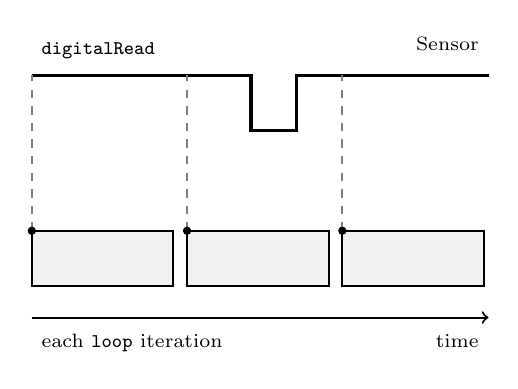
\begin{tikzpicture}[
                x=.58cm, y=.58cm,
                signal/.style={line width=.4mm},
                iter/.style={line width=.25mm, fill=black!5},
                readline/.style={dashed, draw=gray, line width=.25mm},
                lbl/.style={font=\scriptsize},
            ]
                %% the sensor: normally HIGH, briefly LOW as the magnet passes
                \node[lbl, anchor=east] at (10, 5.3) {Sensor};
                \draw[signal] (0, 4.6) -- (4.8, 4.6) -- (4.8, 3.4)
                    -- (5.8, 3.4) -- (5.8, 4.6) -- (10, 4.6);

                %% the pin is only read at the start of each iteration
                \node[lbl, anchor=south west] at (0, 4.75) {\texttt{digitalRead}};
                \foreach \s in {0, 3.4, 6.8}{
                    \draw[iter] (\s, 0) rectangle ++(3.1, 1.2);
                    \draw[readline] (\s, 1.2) -- (\s, 4.6);
                    \filldraw (\s, 1.2) circle (1.3pt);
                }

                %% time
                \draw[->, line width=.25mm] (0, -0.7) -- (10, -0.7);
                \node[lbl, anchor=north east] at (10, -0.85) {time};
                \node[lbl, anchor=north west] at (0, -0.85) {each \texttt{loop} iteration};
            \end{tikzpicture}
            \caption{The pin is only read at the start of each iteration, so a magnet that comes and goes in between is never seen.}
            \label{fig:polling}
        \end{subfigure}
        \hfill
        \begin{subfigure}[t]{.46\textwidth}
            \centering
            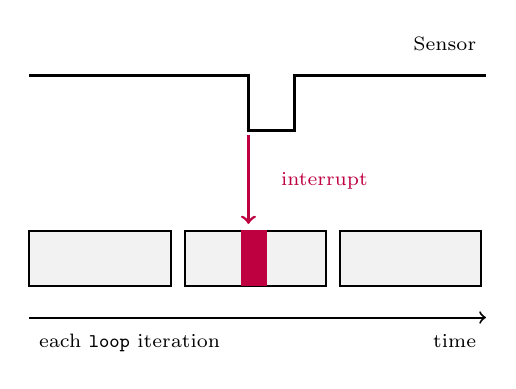
\begin{tikzpicture}[
                x=.58cm, y=.58cm,
                signal/.style={line width=.4mm},
                iter/.style={line width=.25mm, fill=black!5},
                lbl/.style={font=\scriptsize},
            ]
                %% the same sensor signal
                \node[lbl, anchor=east] at (10, 5.3) {Sensor};
                \draw[signal] (0, 4.6) -- (4.8, 4.6) -- (4.8, 3.4)
                    -- (5.8, 3.4) -- (5.8, 4.6) -- (10, 4.6);

                \foreach \s in {0, 3.4, 6.8}{
                    \draw[iter] (\s, 0) rectangle ++(3.1, 1.2);
                }

                %% the falling edge interrupts the loop the moment it happens
                \filldraw[fill=purple, draw=purple] (4.65, 0) rectangle ++(0.55, 1.2);
                \draw[->, line width=.35mm, draw=purple] (4.8, 3.3) -- (4.8, 1.35);
                \node[lbl, anchor=west, text=purple] at (5.3, 2.3) {interrupt};

                %% time
                \draw[->, line width=.25mm] (0, -0.7) -- (10, -0.7);
                \node[lbl, anchor=north east] at (10, -0.85) {time};
                \node[lbl, anchor=north west] at (0, -0.85) {each \texttt{loop} iteration};
            \end{tikzpicture}
            \caption{The falling edge calls the interrupt function straight away, whatever the `loop' function was in the middle of.}
            \label{fig:interrupt}
        \end{subfigure}
    \end{center}
    \caption{Two ways of reading a pin whose value can change at any moment.}
    \label{fig:reading-a-pin}
\end{figure}

Because being able to interrupt the `loop' function is a special case, there may be restrictions (depending on which Arduino you have) as to which pins this feature is enabled on (\url{https://docs.arduino.cc/language-reference/en/functions/external-interrupts/attachInterrupt/}). On the Nano Every, any digital pin can be used; in this lab we will use pin D2.

\section{Creating the circuit}
\label{sec:circuit}
There are two circuits needed for this worksheet, the first is for the hall effect sensor (HES), and the second is for the visual display LED.\\
\textbf{HES circuit}: Arduino +5V\textrightarrow\hspace{0.1em}HES left leg, Arduino GND\textrightarrow\hspace{0.1em}HES middle leg, Arduino Pin D2\textrightarrow\hspace{0.1em}HES right leg. HES left\textrightarrow \hspace{0.1em}$10K\Omega$ resistor\textrightarrow\hspace{0.1em}HES right legs.\\
\textbf{LED circuit}: Arduino Pin D4\textrightarrow $220\Omega$ resistor\textrightarrow LED\textrightarrow Arduino GND.


\section{System Functionality}
\label{sec:functionality}
The basis of this system is that we have an LED and a hall effect sensor --- say placed near the crank or forks of a bike --- connected to our Arduino as described in Section \ref{sec:circuit}. We set up the LED as we did in Lab 2 (but on a different pin) and then attach an interrupt to the pin connected with the hall effect sensor. Every time a magnet passes past the field of the hall effect sensor --- say a magnet on the crank arm of a bike --- the associated interrupt code is called, and it records the time in milliseconds of that event. Within the `loop' function, we can then calculate if the last time the interrupt happened, is  within a 500-millisecond window of the current time. If true, we can turn on the LED, if false, we turn off the LED.

The first thing we need to do is create a blank sketch, this is done by opening Arduino IDE, going to `File'\textrightarrow `Examples'\textrightarrow `01.Basics'\textrightarrow `BareMinimum'. Once this has opened, we can now start to code up the system.

The code within this section should all be placed within the global scope. Like our previous labs, the first piece of code included is defining the external pins and our constants. In our scenario, this is declaring \verb|CRANK_PIN| for our hall effect sensor, and then \verb|CRANK_ACTIVITY_LED_PIN| for our visual feedback as to when the hall effect sensor has been triggered. The last part of code is defining the 500-millisecond window in which we will activate the LED:
% not pulled from the sketch: these sit in two separate blocks with
% explanatory comments between them
\begin{minted}{arduino}
#define CRANK_PIN 2
#define CRANK_ACTIVITY_LED_PIN 4
#define CRANK_PASS_ACTIVITY_DELAY 500
\end{minted}
\vspace{.75em}

Next, we need two global variables: \verb|current_loop_time| to store a consistent execution time in milliseconds across the `loop' function, and \verb|crank_interrupt_current_time| to store the time in milliseconds of the last recorded interrupt:
\inputminted[
    autogobble, stripnl,
    rangestartstring={unsigned long current_loop_time;},
    rangestopstring={volatile unsigned long crank_interrupt_current_time;},
]{arduino}{../lab-4-hall-effect-sensor.ino}
\vspace{.75em}

\textit{Note:} \verb|crank_interrupt_current_time| is marked \verb|volatile| because it is written by the interrupt rather than by the `loop' function. That keyword tells the compiler that the value can change at any moment, so it must be read from memory every time instead of being kept in a register. \verb|current_loop_time| is only ever written by the `loop' function, so it does not need it.

\textit{Note:} The reason we need to store a consistent time across the `loop' function is that a full iteration of the `loop' function takes around 50 milliseconds. If you request the current time (using the \verb|millis()| function we use below) at the beginning of the code, compared to the end of the code, you would get a different value; therefore, to ensure you have a consistent `current time' across an iteration of the `loop' function, you store the value at the beginning of the iteration and then use that referenced value throughout the function.

\section{Setup function}
The code required for the setup function can be thought of as four steps: 1 - enable debugging tools, 2 - initialise global values, 3 - set the pins to the correct modes and attach the interrupt, 4 - pause, then report that the system is ready. The code in the following sections goes into the `setup' function, in the order shown.

\subsection{Enable debugging tools}
As in the previous labs, the first thing to do is start the serial connection so that we can monitor what the Arduino is doing (\textit{hint:} see the `Set up debugging' section of Lab 3):
\inputminted[
    autogobble, stripnl,
    rangestartstring={Serial.begin(9600);},
    rangestopstring={Serial.begin(9600);},
]{arduino}{../lab-4-hall-effect-sensor.ino}
\vspace{.75em}

\subsection{Initialise global variables}
Both of the global system variables (\verb|current_loop_time| and \verb|crank_interrupt_current_time|) have been created but have not been initialised; they exist, but they haven't been given any initial value. As both of these variables hold a time in milliseconds, a logical value for initialisation would be zero (the first possible valid value):
\inputminted[
    autogobble, stripnl,
    rangestartafterstring={// set default values},
    rangestopbeforestring={// setup LED pin as output},
]{arduino}{../lab-4-hall-effect-sensor.ino}
\vspace{.75em}

\subsection{Pins}
Next within the `setup' function, we set up the pins. The LED pin needs to be set to mode \verb|OUTPUT| and then to ensure the LED isn't already on, write to the LED a \verb|LOW| value to turn it off. Next, the hall effect sensor pin needs to be set to mode \verb|INPUT| and an interrupt needs to be added to the pin. In code terms, the interrupt is a separate function that is only called when the interrupt is triggered. In our code, this is a function called \verb|crankInterrupt| that we define in the next section of the worksheet. All we are doing in the `setup' function, is referencing the \verb|crankInterrupt| function, we do not create the function itself.

There are several options when you attach the interrupt to define when the interrupt function is called. In our case we are using the \verb|FALLING| mode (\url{https://docs.arduino.cc/language-reference/en/functions/external-interrupts/attachInterrupt/#parameters}) as our hall effect sensors report a \verb|HIGH| value when no magnet is present, and the value then drops when a magnet is present:
\inputminted[
    autogobble, stripnl,
    rangestartafterstring={crank_interrupt_current_time = 0;},
    rangestopbeforestring={// pause the system},
]{arduino}{../lab-4-hall-effect-sensor.ino}
\vspace{.75em}

\subsection{System ready}
The last thing to do in the `setup' function is to pause the system for 3 seconds, and then display the message `System Ready' in the serial monitor:
\inputminted[
    autogobble, stripnl,
    rangestartafterstring={// pause the system},
    rangestopstring={Serial.println("System Ready");},
]{arduino}{../lab-4-hall-effect-sensor.ino}
\vspace{.75em}

\section{Interrupt}
As discussed above, we need a new function that appears in the global scope (like the `setup' \& `loop' function) which can be called by the interrupt attached to the hall effect sensor pin. All this method does is record the current time in milliseconds to the \verb|crank_interrupt_current_time| variable. As an interrupt is stopping everything else running on an Arduino, you try to keep the code inside the interrupt to the bare minimum required: in our case, this is simply recording the time. All the intensive computational logic is done within the `loop' function --- determining if the LED should be on and thus turning on or off the LED.
\inputminted[
    autogobble, stripnl,
    rangestartstring={void crankInterrupt()},
]{arduino}{../lab-4-hall-effect-sensor.ino}
\vspace{.75em}

\section{Loop function}
The main logic of the loop can be divided into two steps: 1 - calculate if the last occurrence of the interrupt is within the 500-millisecond window, 2 - wait.

\subsection{Calculate window}
The first part for calculating the window is storing into the \verb|current_loop_time| variable the current time in milliseconds. Next, you calculate if the current time and the last occurrence of the interrupt are within the 500-millisecond window. If true, you turn on the LED with the standard \verb|digitalWrite| method. We also then display a debug message so that if the LED isn't working, we can still see that the logic in the Arduino is working correctly. Because the `loop' function runs every 50 milliseconds, expect this message to repeat many times for each pass of the magnet. If the window has passed, we turn off the LED:
\inputminted[
    autogobble, stripnl,
    rangestartafterstring={// display the crank activity LED},
    rangestopbeforestring={// delay the system},
]{arduino}{../lab-4-hall-effect-sensor.ino}
\vspace{.75em}

\subsection{Wait}
The final logic within the `loop' function is to wait 50 milliseconds before the next iteration of the `loop' function:
\inputminted[
    autogobble, stripnl,
    rangestartstring={delay(50);},
    rangestopstring={delay(50);},
]{arduino}{../lab-4-hall-effect-sensor.ino}
\vspace{.75em}

\section{Try it out on your Arduino}
You now should be able to compile your sketch (`Sketch'\textrightarrow `Verify/Compile') and then upload to your Arduino (`Sketch'\textrightarrow `Upload'). You should now be able to pass the magnet across a side of the hall effect sensor, and every time you do, it should light up the LED. \textit{Note:} the hall effect sensors are directional, so if the LED isn't lighting up, turn over the magnet and try again.

\section{Extension}
Imagine your Hall effect sensor is mounted on the fork of a bike and the magnet is attached to one of the spokes, so that the magnet passes the sensor once per turn of the wheel. Taking the radius of a 700c road wheel to be $0.34$\,m, extend your code to compute the bike speed as the magnet passes and print this to the serial monitor. Pass the magnet in front of the sensor several times to simulate the spinning of the wheel, see if you can make the speed rise and fall by changing the frequency of the magnet passing the sensor. A computation like this will be the basis of the control system we build in the next three weeks.

As a challenging extra, see if you can create a `speedometer' by writing to a servomotor on another pin. Let 0 degrees correspond to zero speed and 180 degrees to the maximum permitted speed of an e-bike in the UK.  

\pagebreak
\section*{Help}
If you are having issues compiling the project or don't understand where each section goes, you can see a complete version of the sketch with additional source code comments at \url{https://github.com/MDCHAMP/MAC233/blob/main/labs/lab-4-hall-effect-sensor/lab-4-hall-effect-sensor.ino}.

\begin{center}
    \qrcode[hyperlink, height=4cm]{https://github.com/MDCHAMP/MAC233/blob/main/labs/lab-4-hall-effect-sensor/lab-4-hall-effect-sensor.ino}
\end{center}

\vspace{2em}

Additionally, if you are wondering how the components connect together, the circuit diagram for this lab is below.

\begin{center}
    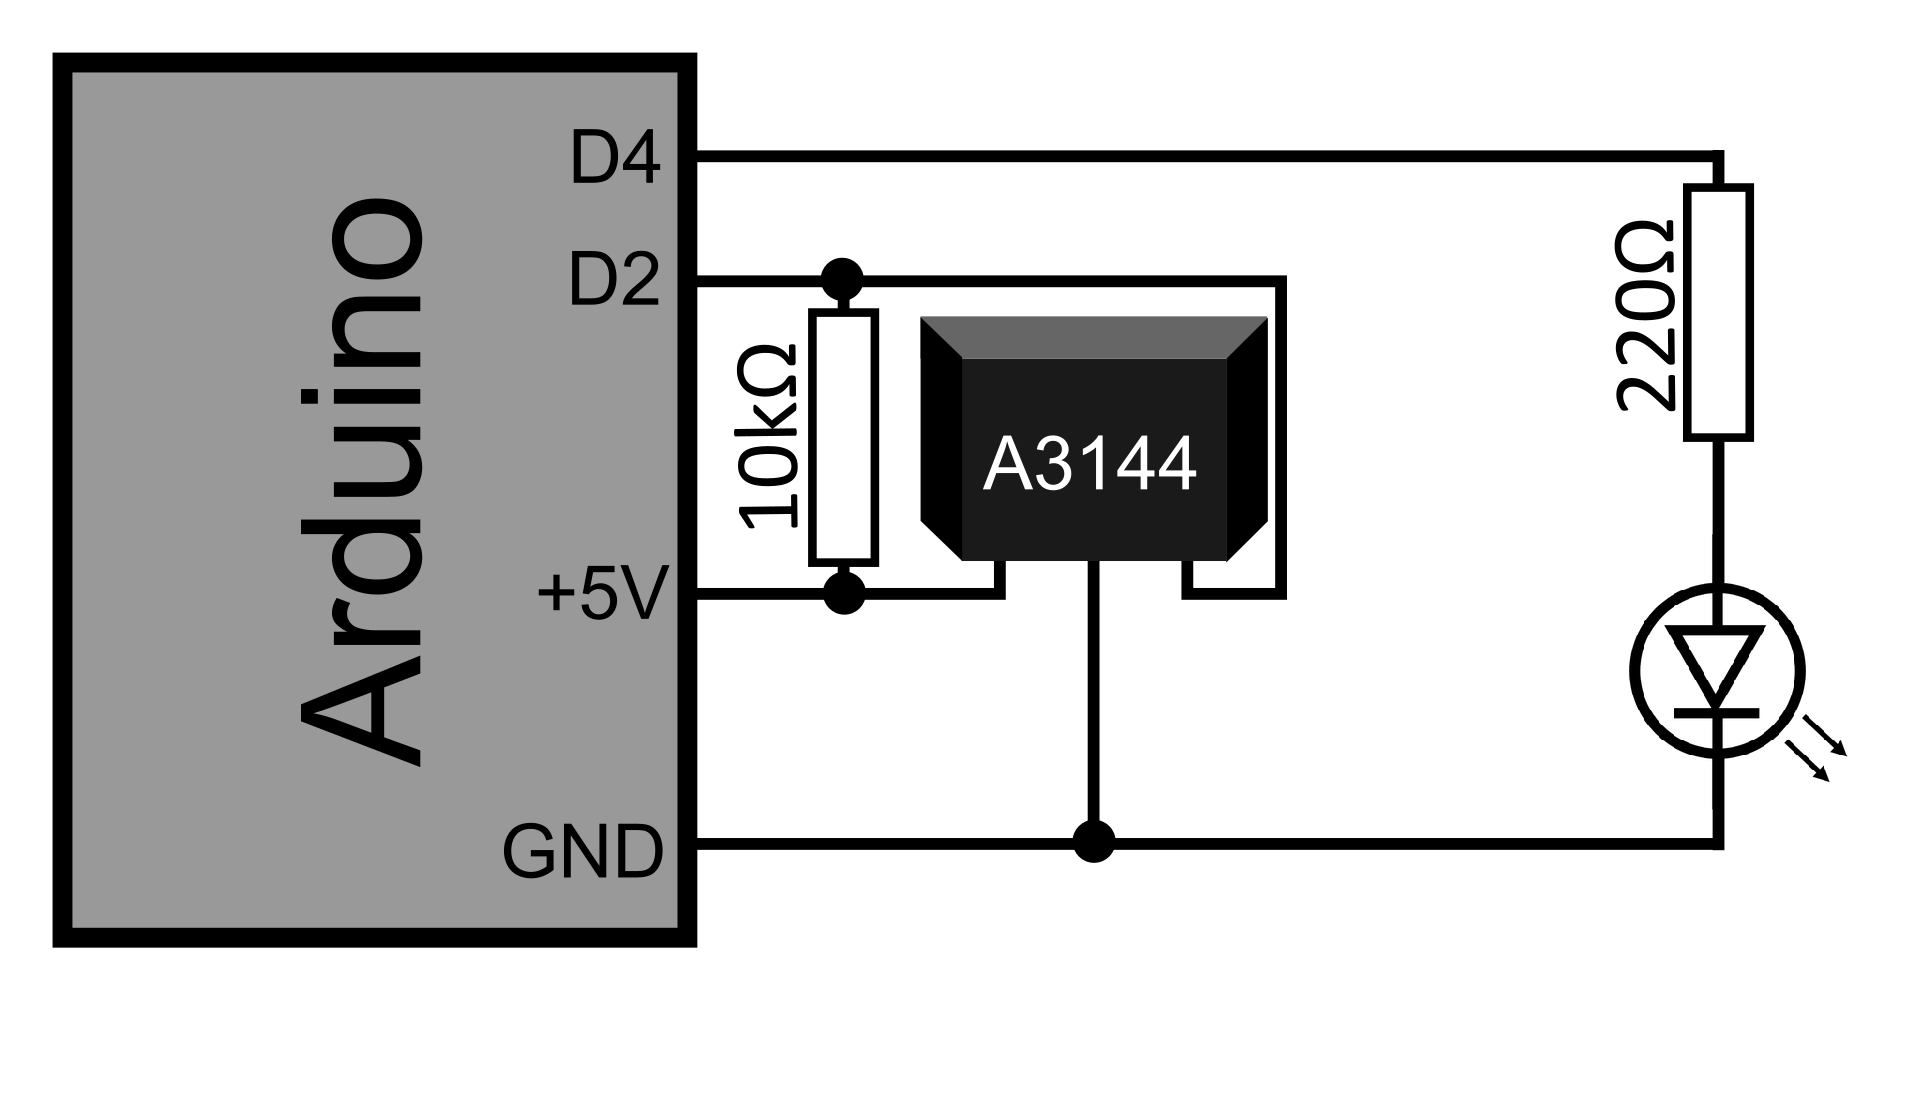
\includegraphics[width=.6\textwidth]{../images/wiring-diagram.png}
\end{center}

\end{document}